\section{Results}

Current results include the generation of time series data to be used in
training the RC model. Shown in Figure \ref{fig:demand}, Figure \ref{fig:solar}, and Figure \ref{fig:wind}.

\begin{figure}[h]
 	\centering
 	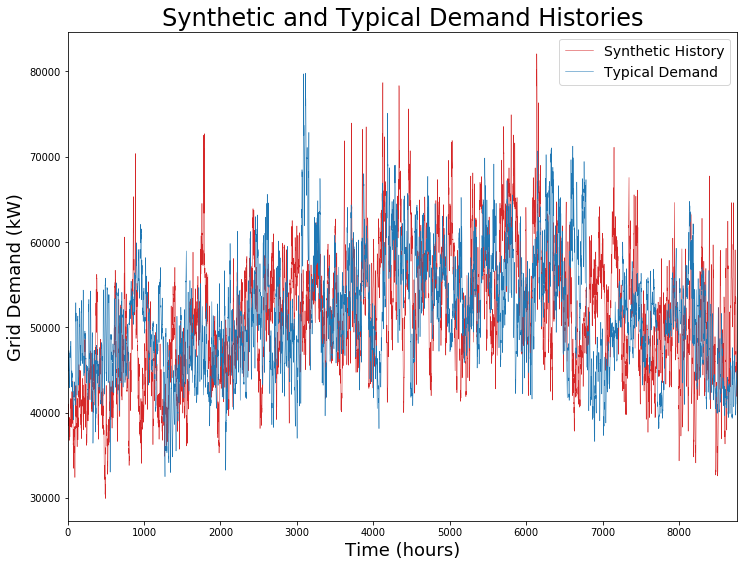
\includegraphics[width=0.8\columnwidth]{syn_typ_demand.png}
 	\caption{The typical year of hourly grid demand in kW at UIUC.}
  \label{fig:demand}
\end{figure}
\begin{figure}[h]
	\centering
	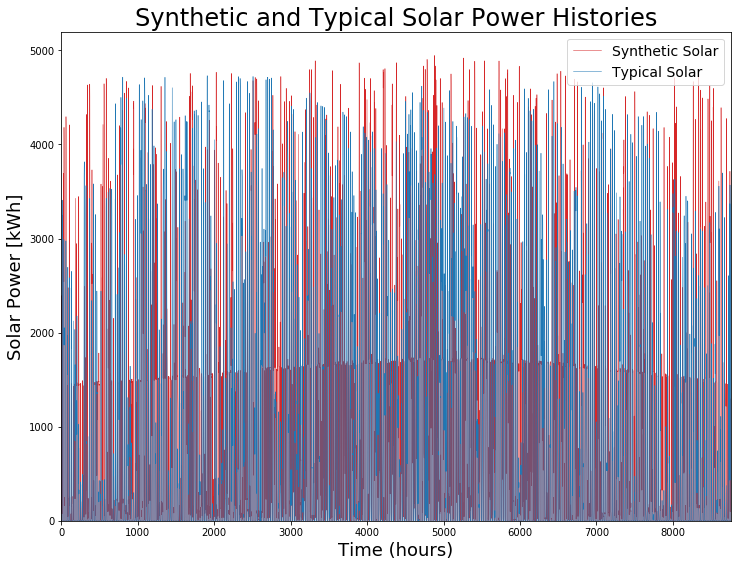
\includegraphics[width=0.8\columnwidth]{syn_typ_solar.png}
	\caption{The typical year and a synthetic year of hourly solar electricity
  \label{fig:solar}
  generation in kWh per hour at UIUC. Data from
  \cite{alsoenergy_university_2019}}
\end{figure}
\begin{figure}[h]
	\centering
	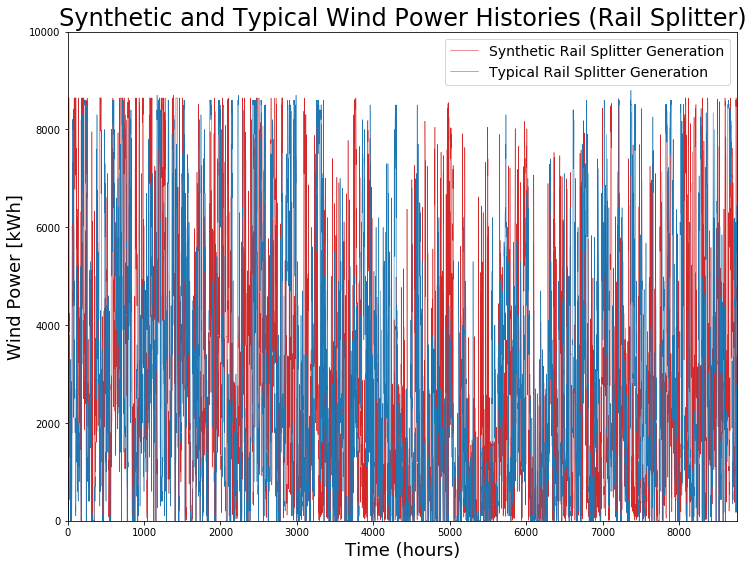
\includegraphics[width=0.8\columnwidth]{syn_typ_railsplitter.png}
	\caption{The typical year and a synthetic year of hourly power produced by
  \label{fig:wind}
  the UIUC wind power purchase agreement with Railsplitter Wind Farm.}
\end{figure}

The hyperparameters of the \acrshort{ESN} used in Figure \ref{fig:ESN1} and
Figure \ref{fig:ESN2} have not been optimized. In spite of this, preliminary
predictions track reasonably well with grid demand. We conducted a single grid
search for the an optimal combination of spectral radius ($\rho$) and noise
injection (for regularization of reservoir neurons), Figure
\ref{fig:gridsearch}, following the recommendations from
\cite{lukosevicius_practical_2012}.

\begin{figure}[h]
  \centering
  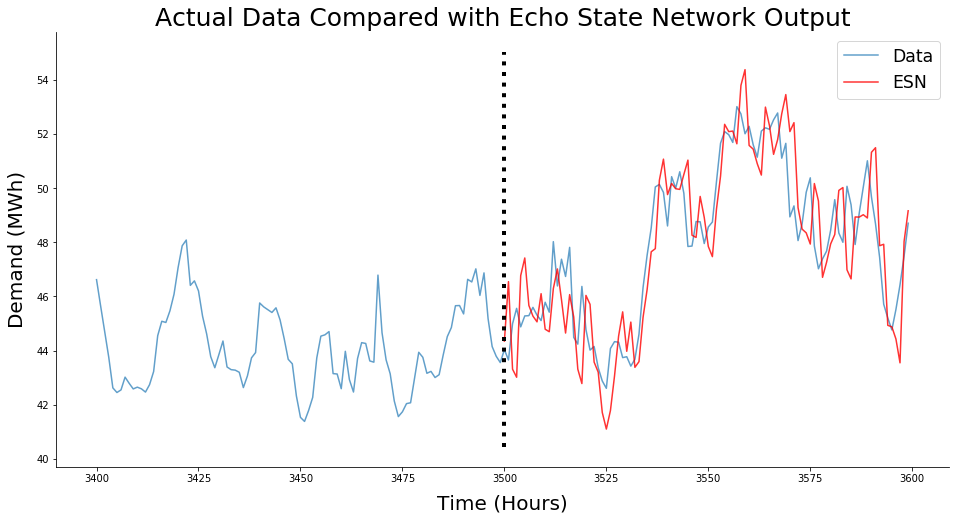
\includegraphics[width=\columnwidth]{scaled_esn_network.png}
  \caption{A simple ESN with a prediction of 100 hours into the future. After
  training on 1000 hours of historical data.}
  \label{fig:ESN1}
\end{figure}
\begin{figure}[h]
  \centering
  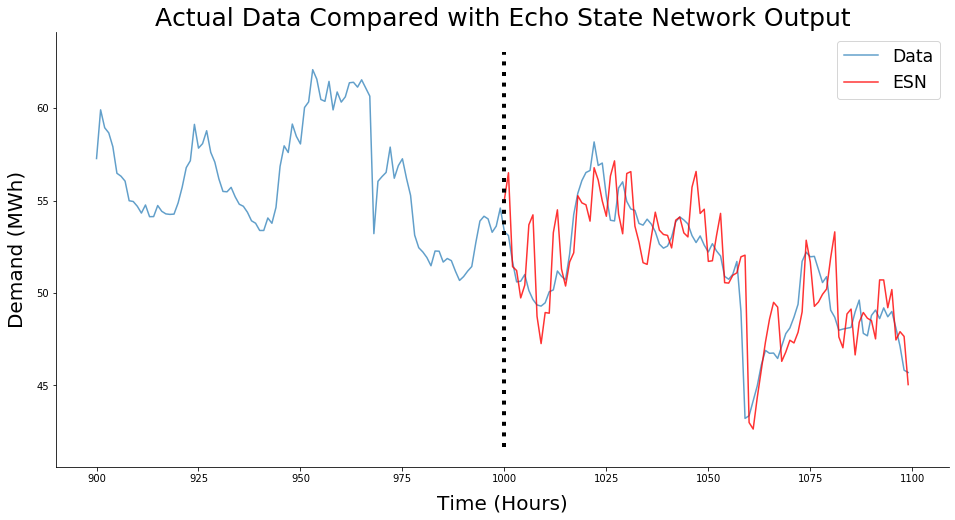
\includegraphics[width=\columnwidth]{scaled_esn_network2.png}
  \caption{A simple ESN with a prediction of 100 hours into the future after
  training on 3500 hours of historical data.}
  \label{fig:ESN2}
\end{figure}
\begin{figure}[h]
  \centering
  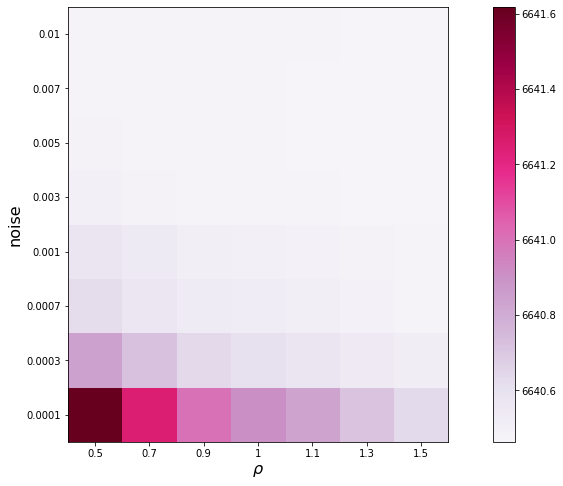
\includegraphics[width=0.8\columnwidth]{noise_spectral_radius.png}
  \caption{A grid search over a range of spectral radii and noise levels. The
  optimal set minimizes the mean squared error.}
  \label{fig:gridsearch}
\end{figure}
